\documentclass[../thesis.tex]{subfiles}

\begin{document}
In this appendix we discuss software and computational aspects of the analysis presented in Chapter~\ref{chap:tmb_estimation}.
\section{R package \texttt{ICBioMark}\label{sec:icbiomark}}
In this section we'll demonstrate use of the R package \texttt{ICBioMark} \citep{bradley_icbiomark_2021} on a toy example containing simulated data. The same core workflow, applied to real data, will form almost all of the results described throughout the remained of the chapter.

The package \texttt{ICBioMark} is available via the R repository CRAN and so can be installed and loaded with:
\begin{lstlisting}
    install.packages(`ICBioMark')
    library(ICBioMark)
\end{lstlisting}
or from GitHub with:
\begin{lstlisting}
    install.packages(`devtools') 
    devtools::install_github(`cobrbra/ICBioMark')
    library(ICBioMark)
\end{lstlisting}
(note that the GitHub version is development and may not be as stable as the CRAN release, but may contain more features). The toy dataset we use here comes pre-loaded with the package, but just comes from the data simulation function \lstinline{generate_maf_data()}, which allows for a variety of choices of dataset size and shape.

Our example dataset, called \lstinline{example_maf_data}, is a list with two elements: \lstinline{maf} and \lstinline{gene_lengths}. These two pieces of data are required for most of the tasks performed by \texttt{ICBioMark}. They are organised as follows:
\begin{enumerate}
    \item The dataset \lstinline{maf} is a data frame in \glsxtrlong{maf}. For a set of sequenced tumour/normal pairs, this means a table with a row for every mutation identified, with columns corresponding to properties such as the sample ID for the tumour of origin, the gene, chromosome and nucelotide location of the mutation, and the type of mutation observed. In the real world, \glsxtrshort{maf} datasets often have lots of extra information beyond this, but for our example we only include sample, gene and mutation type. See the first five rows in Table~\ref{tab:example_maf} -- generating code below: 
\begin{lstlisting}
    head(example_maf_data$maf, 5)
\end{lstlisting}
\begin{table}[hb]
    \centering
    \begin{tabular}{c|c|c}
         \verb|Tumor_Sample_Barcode| & \verb|Hugo_Symbol| & \verb|Variant_Classification| \\
         \hline
\verb|SAMPLE_96| &	\verb|GENE_14|	& \verb|Missense_Mutation| \\
\verb|SAMPLE_73| &	\verb|GENE_14| & \verb|Frame_Shift_Ins| \\
\verb|SAMPLE_55| &	\verb|GENE_4| & \verb|Missense_Mutation| \\
\verb|SAMPLE_96| &	\verb|GENE_3| & \verb|Missense_Mutation| \\
\verb|SAMPLE_38| &	\verb|GENE_7| & \verb|Missense_Mutation| \\
    \end{tabular}
    \caption{First five rows of \lstinline{example_maf_data$maf}.}
    \label{tab:example_maf}
\end{table}

    \item The data frame \lstinline{gene_lengths} contains the names (referred to by Hugo Symbol) of genes to be included in downstream modelling, alongside their length. As discussed above, gene length is a complex and subtle quantity to define -- we advise using coding length as defined in the \emph{Ensembl} database \citep{yates_ensembl_2020}. For this example, however, gene lengths are again randomly chosen by the simulating function. Example rows are given in Table~\ref{tab:example_gene_lengths} with accompanying code snippet below: 
\begin{lstlisting}
    head(example_maf_data$gene_lengths, 5)
\end{lstlisting}
\begin{table}[ht]
    \centering
    \begin{tabular}{c|c}
         \verb|Tumor_Sample_Barcode| & \verb|Hugo_Symbol| \\
         \hline
\verb|GENE_1| &	961	\\
\verb|GENE_2| &	1009  \\
\verb|GENE_3| &	1011  \\
\verb|GENE_4| &	976 \\
\verb|GENE_5| &	1016\\
    \end{tabular}
    \caption{First five rows of \lstinline{example_maf_data$gene_lengths}.}
    \label{tab:example_gene_lengths}
\end{table}
\end{enumerate}
 User-provided gene length datasets, which we recommend extracting from the \emph{Ensembl} database \citep{yates_ensembl_2020}, are permitted to contain values for more genes than are observed in the accompanying \gls{maf} dataset. In general, if a few genes covered by a \gls{wes} experiment are missing gene length information it will not drastically impact model performance, but lots of missing values will begin to cause issues with model accuracy. Later versions of this \texttt{ICBioMark} will address missing gene length data.

In our next step we specify training/validation/test split and build model matries. The \gls{maf} format is widely used and standardised, but not especially helpful for sample(/patient)-level prediction. The ideal format for our data is a matrix in which every row corresponds to a sample, every column corresponds to a gene/mutation type combination, and each entry corresponds to how many mutations in that sample, gene and type were identified by sequencing. At the same time as this, we’d like to separate our training data from separately reserved validation and test data. We do this using the function \lstinline{get_mutation_tables()}.

Our procedure, described in Section~\ref{sec:genmodel}, models different mutation types separately, so in theory one could have separate parameters for each mutation type (e.g. \texttt{`Missense\_Mutation'} or \texttt{`Frame\_Shift\_Ins'}). However, doing so would vastly increase the computational complexity of fitting a generative model. It is also not particularly informative to fit parameters to extremely scarce mutation types. Mutations types are grouped and filtered by the function \lstinline{get_mutation_dictionary()}. In general we recommend separately modelling indel mutations (so that we can predict \gls{tib} later), synonymous mutations (as these don’t count towards \gls{tmb} or \gls{tib}), and grouping together all other nonsynonymous mutation types. The function \lstinline{get_mutation_dictionary()} allows for the production of a list of mutation types, with labels for their groupings.

Next we produce our training, validation and test sets. Again, for this example workflow these are availbale pre-loaded, but can also be produced with the \lstinline{`get_mutation_tables'} function. The object produced has three elements: \lstinline{`train'}, \lstinline{`val'} and \lstinline{`test'}. Each of these contains a sparse mutation matrix (\lstinline{`matrix'}) and other information describing the contents of the matrix (\lstinline{`sample_list'}, \lstinline{`gene_list'}, \lstinline{`mut_types_list'}, and \lstinline{`col_names'}). See example code below.

\begin{lstlisting}
    example_tables <- get_mutation_tables(
        example_maf_data$maf,
        sample_list = paste0("SAMPLE_", 1:100)
    )
    print(head(example_tables$train$col_names, 10))
>  [1] `GENE_1_NS' `GENE_1_I'  `GENE_1_I'  `GENE_2_NS' 
>  [5] `GENE_2_I'  `GENE_2_S'  `GENE_3_NS' `GENE_3_I'  
>  [9] `GENE_3_S'  `GENE_4_NS'
\end{lstlisting}

At this point we are ready to fit a generative model, for which we need only to provide gene lengths data and training data to the function \lstinline{fit_gen_model()}. We can visualise output of our model with \lstinline{vis_model_fit()} (see Figure~\ref{fig:readme_example_gen_model}). Since this is a small example, we don’t get a particularly strong signal, but we do see an optimum level of penalisation.
\begin{lstlisting}
    example_gen_model <- fit_gen_model(
        gene_lengths = example_maf_data$gene_lengths, 
        table = example_tables$train
    )

    print(vis_model_fit(example_gen_model))
\end{lstlisting}
\begin{figure}[htbp]
    \centering
    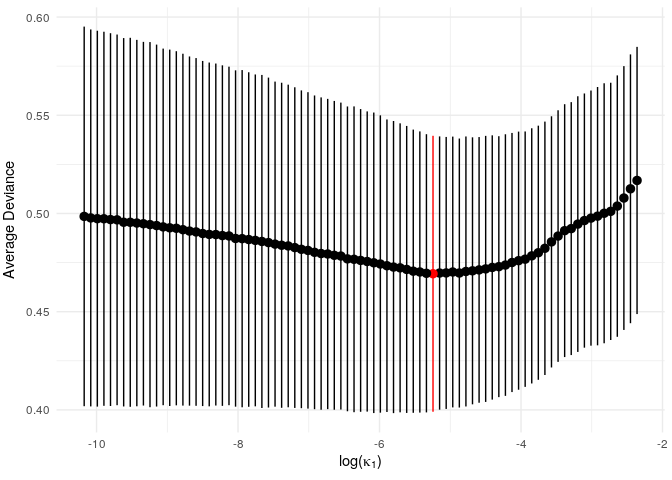
\includegraphics[width=4in]{figures/chapter3/README-example_gen_model-1.png}
    \caption{Output example showing the variation in cross-validated generative model fit for a model fitted to example simulated data.}
    \label{fig:readme_example_gen_model}
\end{figure}
We now construct a first-fit predictive model. The parameter \lstinline{lambda} controls the sparsity of each iteration, so it may take some experimentation to get a good range of panel lengths. From this, we can construct a range of refit estimators.
\begin{lstlisting}
    example_first_pred_tmb <- pred_first_fit(
        gen_model = example_gen_model, 
        lambda = exp(seq(-9, -14, length.out = 100)),
        training_matrix = example_tables$train$matrix, 
        gene_lengths = example_maf_data$gene_lengths
    )
    example_refit_range <- pred_refit_range(
        pred_first = example_first_pred_tmb, 
        gene_lengths = example_maf_data$gene_lengths
    )
\end{lstlisting}

With a predictive model fitted, we can use the function \lstinline{get_predictions()} along with a new (validation or test) dataset to produce predictions on that dataset. We then provide several functions including \lstinline{get_stats()} to analyse the output compared to true values (example results in Figure~\ref{fig:readme_example_predictions}).
\begin{lstlisting}
    example_refit_range %>% 
        get_predictions(new_data = example_tables$val) %>%
        get_stats(
            biomarker_values = example_tmb_tables$val, 
            model = "T", 
            threshold = 10
        ) %>% 
        ggplot(aes(x = panel_length, y = stat)) + 
            geom_line() + 
            facet_wrap(~metric) + 
            theme_minimal() + 
            labs(
                x = "Panel Length", 
                y = "Predictive Performance"
            )
\end{lstlisting}
\begin{figure}[htbp]
    \centering
    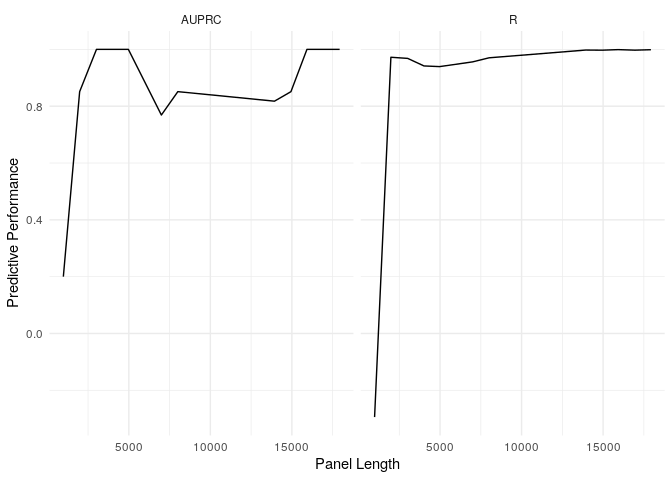
\includegraphics[width=4in]{figures/chapter3/README-example_predictions-1.png}
    \caption{Example prediction summary statistics from \texttt{ICBioMark} estimators applied to simulated data.}
    \label{fig:readme_example_predictions}
\end{figure}
\dobib % renders bibliography (only when compiling for chapter only)
 
\end{document}